%! TEX root = ./main.tex

\lecture{19}{Week 10}{Exception Handling in Processors}
\paragraph{(Exceptional) Control Flow}
While processors do in essence nothing other than processing a stream of instruction, they also have to react to special events like listen for keyboard inputs. 

Jumps and branches, as well as calls and returns are two mechanism which change the control flow based on the program state. But there are also changes to the system state, on which the processor must react. For example data arrival from disk or network, division by zero, user terminates a program or system timers responsible for scheduling. So the system needs to handle \textit{exceptional control flow}.

\textit{Exceptional control flow} exists on all levels of a computer system:
\begin{itemize}
    \item Low Level Mechanisms
        \begin{itemize}
            \item Hardware exception
            \item Combination of HW and OS SW, i.e. malloc
        \end{itemize}
    \item High Level Mechanisms
        \begin{itemize}
            \item Process content switch
            \item Signals, e.g. terminate a program, segmentation fault...
            \item Nonlocal Jumps used for coroutines
            \item Programming language exceptions
        \end{itemize}
\end{itemize}

\paragraph{Exception}
An exception is a transfer of control to the OS in response to some event. It is in essence a context switch. After the OS has handled the exception, the processor switches back to the user process.

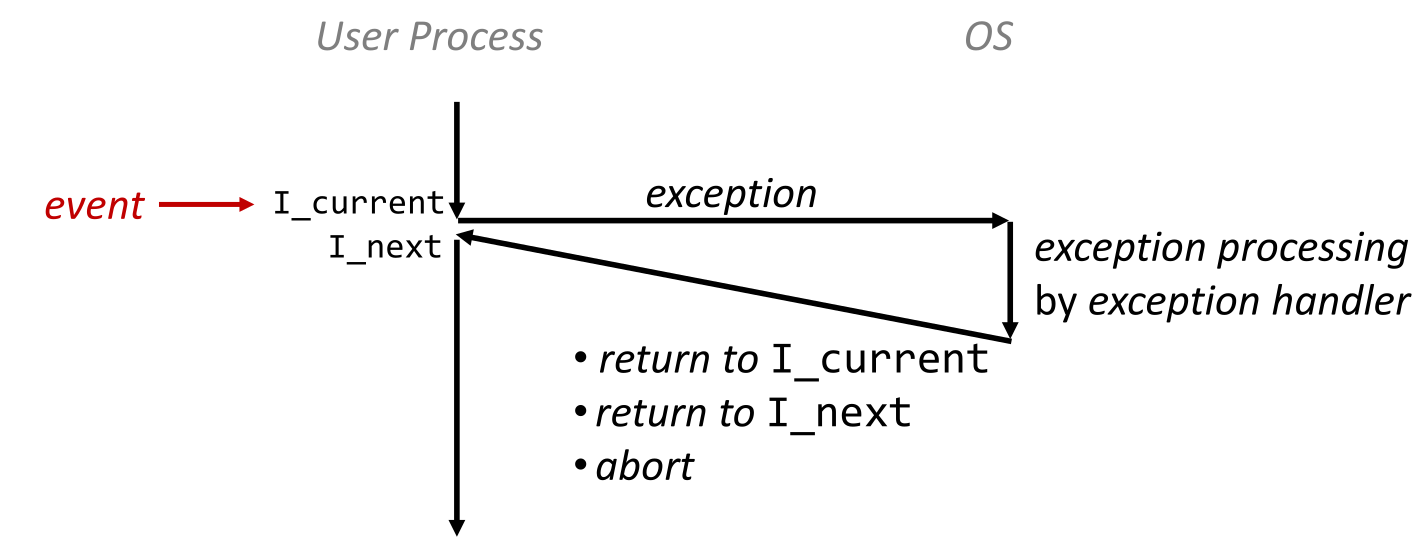
\includegraphics[width=0.8\textwidth]{19_exception.png}

\paragraph{Types of Exceptions}
There are two main types of exceptions:
\begin{description}
    \item[Synchronous Exception:] Result of executing an instruction.
        \begin{description}
            \item[Trap:] Internal exception
            \item[Fault:] Potentially recoverable error
            \item[Abort:] Nonrecoverable error
        \end{description}
    \item[Asynchronous Execption:] Result of an event that are external to the processor.
        \begin{description}
            \item[Interrupt:] Signal from I/O device
        \end{description}
\end{description}

\paragraph{Exception Vector}
At boot time, the OS allocated and initializes the \textit{exception table}. Its base address is stored in the \textit{Exception Table Base Register}. Each type of exception has a unique number $k$, called interrupt vector, which is used to index into the exception table. When exception $k$ occurs, handler $k$ is called.

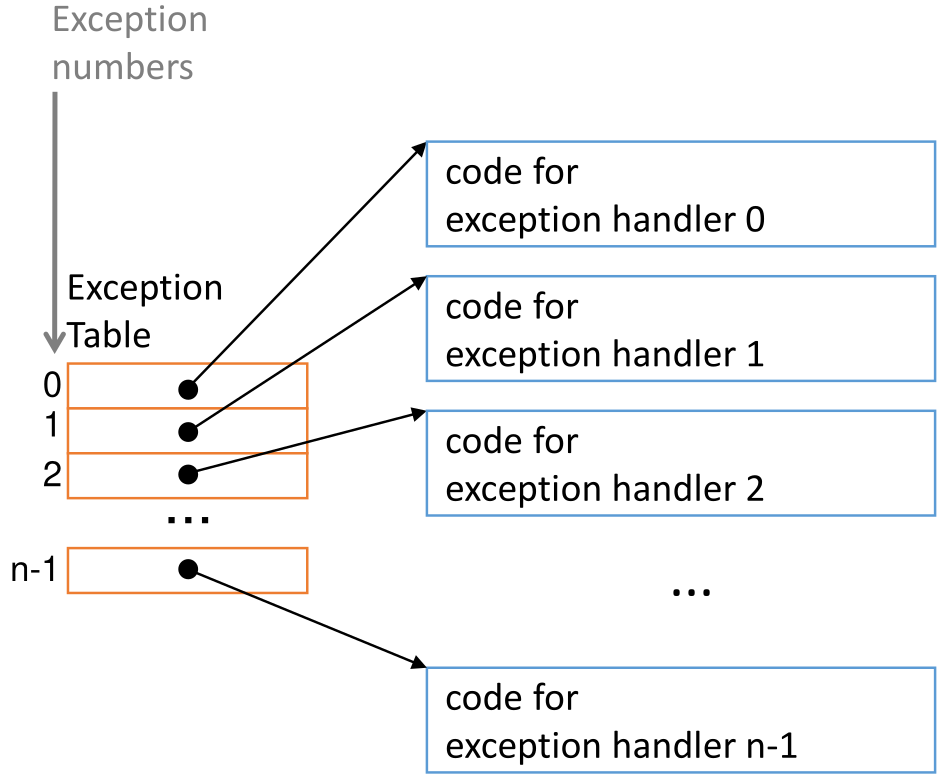
\includegraphics[width=0.8\textwidth]{19_exceptionVector.png}

The exception vectors for x86 are the following:

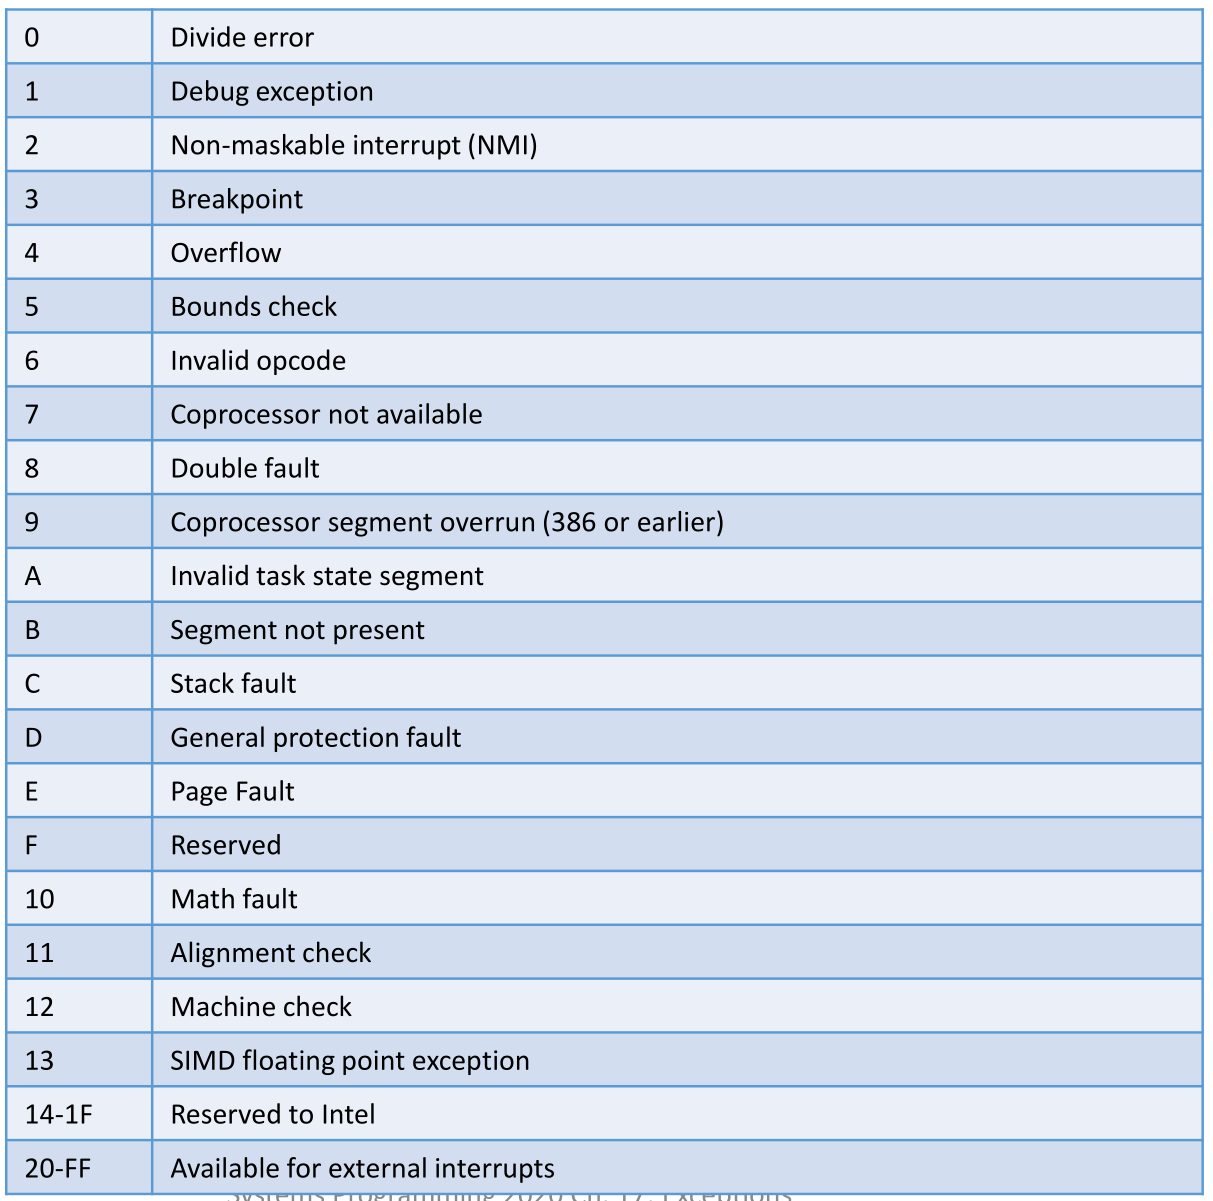
\includegraphics[width=0.8\textwidth]{19_exceptionVectorsx86.png}

\paragraph{Kernel}
Most OS contain a kerne. The kernel is the part of the OS which runs in kernel mode. This means it has some privileges compared the user mode, where programs are run. But on a exception, to content is switched to kernel mode (aka supervisor mode, privileged mode, ring $0$ etc.). In kernel mode a program has access to system states (virtual memory etc.), there are some new instructions and registers available, some exceptions are disabled etc.
I.e. the kernel is always:
\begin{itemize}
    \item a set of trap handling functions
    \item code to create the illusion of user-space processes
\end{itemize}
and sometimes:
\begin{itemize}
    \item a set of threads in a special address space
\end{itemize}

\subsubsection{Synchronous Exceptions}
They are caused by executing instructions.

\begin{description}
    \item[Traps:] 
        \begin{itemize}
            \item Intentional
            \item Returns control to the "next" instruction
            \item Example: system calls, breakpoint traps (while debugging), special instructions
        \end{itemize}
    \item[Faults:]
        \begin{itemize}
            \item Unintentional
            \item Sometimes recoverable
            \item Re-execute faulty ("current") instruction or abort
            \item Example: page fault (recoverable), protection fault (unrecoverable), floating point exception
        \end{itemize}
    \item[Aborts:]
        \begin{itemize}
            \item Unintentional
            \item Unrecoverable
            \item Aborts current program
            \item Example: parity error, machine check
        \end{itemize}
\end{description}

On an exception, the CPU gets the \textbf{exception handler} by indexing into the interrupt exception table using the interrupt vector.

\paragraph{Fault Example: Page Fault}
Code tries to access a location of its address space which is currently not in main memory but on disk. So the page handler must load that page into physical memory. After doing this, it returns to faulting instruction and successfully execute it on the second try.

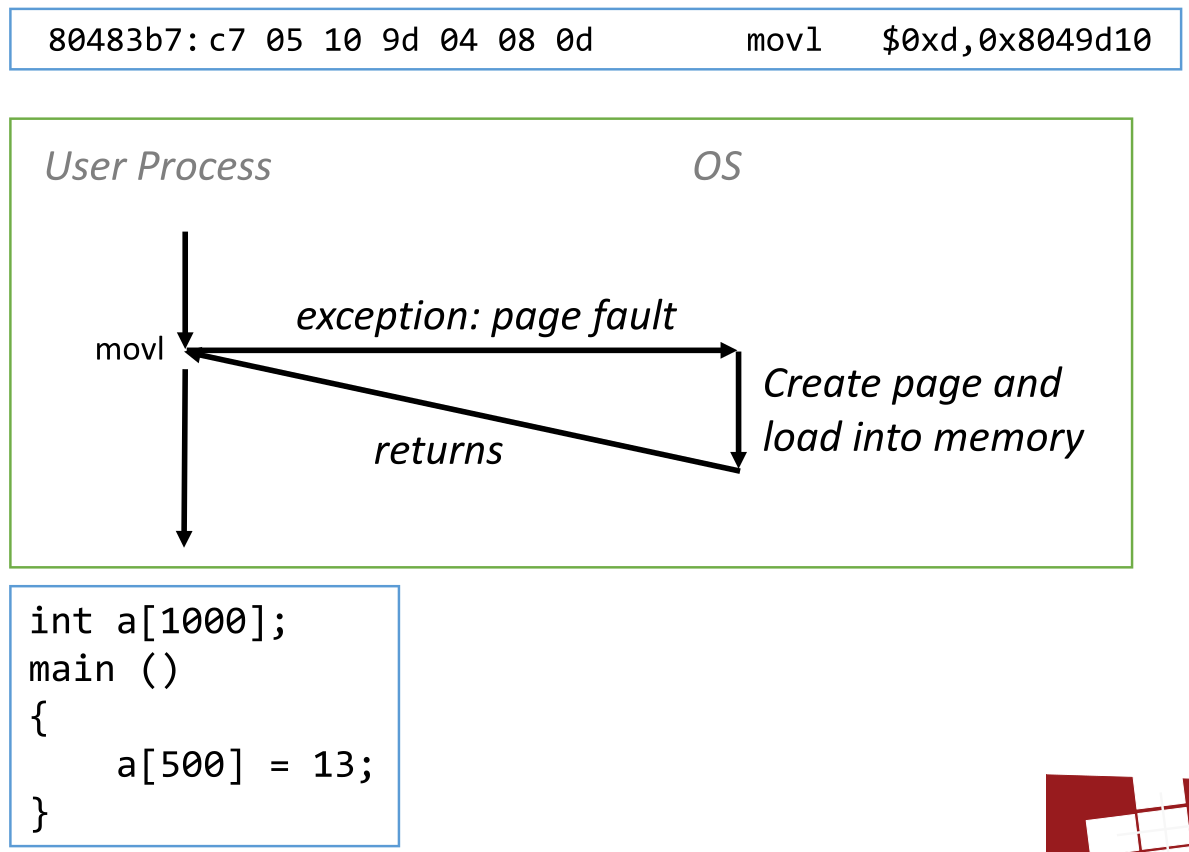
\includegraphics[width=0.8\textwidth]{19_pageFault.png}

\paragraph{Fault Example: Invalid Memory Reference}
Code tries to access a location outside of its address space (i.e. an page which we do not have permissions for). The page handler detects the invalid address and sends a \textbf{SIGSEGV} signal to the user process. The user process exits with \textit{segmentation fault}.

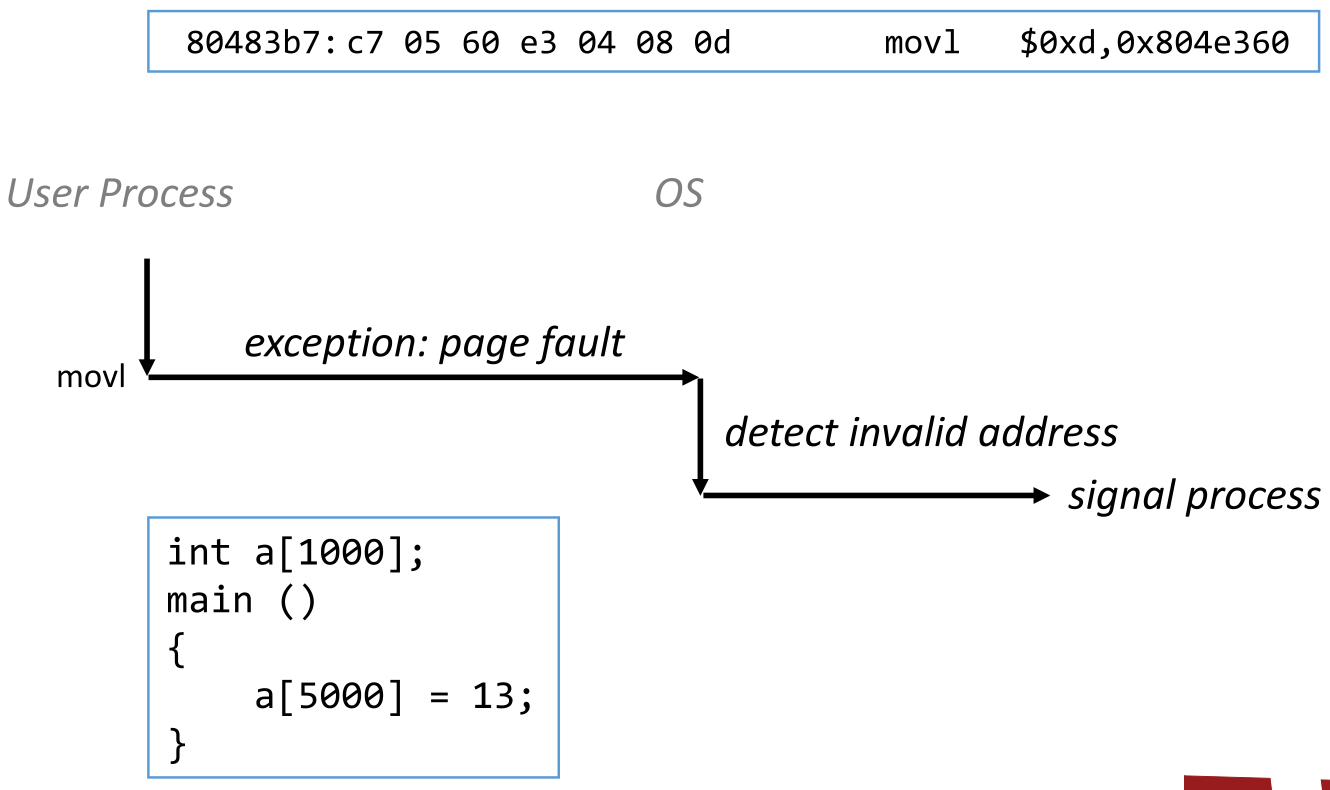
\includegraphics[width=0.8\textwidth]{19_invalidMemoryReference.png}

\paragraph{Trap Example: Opening a File}
User opens a file by calling \code{open(filename, options)} which executes a systems call (e.g. \textit{int} instruction). The OS must find or create the file and get it ready for reading or writing. Then it returns an integer which uniquely defines this file (required for reading the next time the same file).

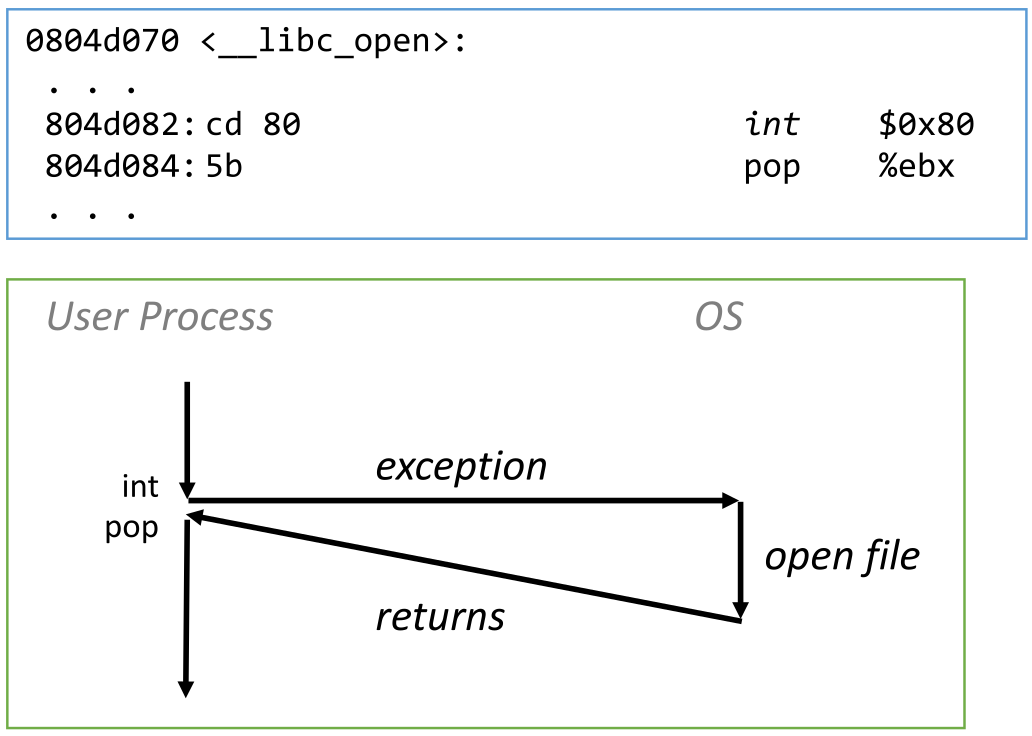
\includegraphics[width=0.8\textwidth]{19_openingAFile.png}

\subsubsection{Asynchronous Exceptions}
They are caused by events external to the processor and indicated to the processor by setting the processor's interrupt pin. The processor finished the current instruction and saves the state before switching to the interrupt.

Examples:
\begin{itemize}
    \item I/O interrupts (keyboard, network packages etc.)
    \item Hard reset interrupts (click power button)
    \item Soft reset interrupts
\end{itemize}

These interrupts pins of the processor are connected to interrupt-request lines. They are either edge- or level-triggered.

Interrupt are either \textbf{maskable} or \textbf{non-maskable}. It they are, then the interrupt can be ignored or delayed. This allows to prioritize certain interrupts over others.

The mechanism for handling interrupts is equivalent to the one of exceptions (index into exception table using exception vector etc...).

\subsubsection{x86 interrupts}
These processors have two interrupt pins:

\paragraph{Non-Maskable Interrupt (NMI)}
Non-maskable means that these interrupts cannot be disabled. So they are used for interrupts of high importance like major hardware faults (e.g. memory parity error), watchdog timer etc.

When asserted, the processor completes the current instruction and then issues the exception \#2 of the exception interrupt table (this is hardcoded).

Since multiple devices are connected to this pin, the exception handler has to figure out which device has cause the interrupt. The OS iterates all possible devices and checks which one has a state which indicates that the device has caused an interrupt. This check is called \textit{pulling} and is something quite inefficient and slow. However, since we are very likely to crash anyways, it is not something that happens very often.

NMI does not support nesting. This means that when processing a first interrupt the processor does not listen for any new interrupts which may occurs in the meantime. 

\paragraph{Interrupt Request (INTR)}
These requests can be disabled by setting certain bit (flags). If asserted, the processor completes the current instruction and saved the state, then it acknowledges the receive by setting the INTA pin. The device detects that and in consequence sends the interrupt vector to the processor via the data bus. The processor issues the designated exception handler. 

\subsubsection{Interrupt Controllers}
Using the introduces setup, we have to problem that a device does not know what vector to give. Also, it may cause troubles when multiple devices cause an interrupt at the same time.

\paragraph{Programmable Interrupt Controller (PIC)}
The PIC solves these problem. It is a device which is connected to the INTR pin and the data bus of the processor. Further, all devices are no longer connected to the processor directly, but to the PIC via IRQ-lines. This way, the OS can flexibly configure what vector to send on what interrupt of which device. I.e. the PIC maps interrupt pins from devices to interrupt vectors.

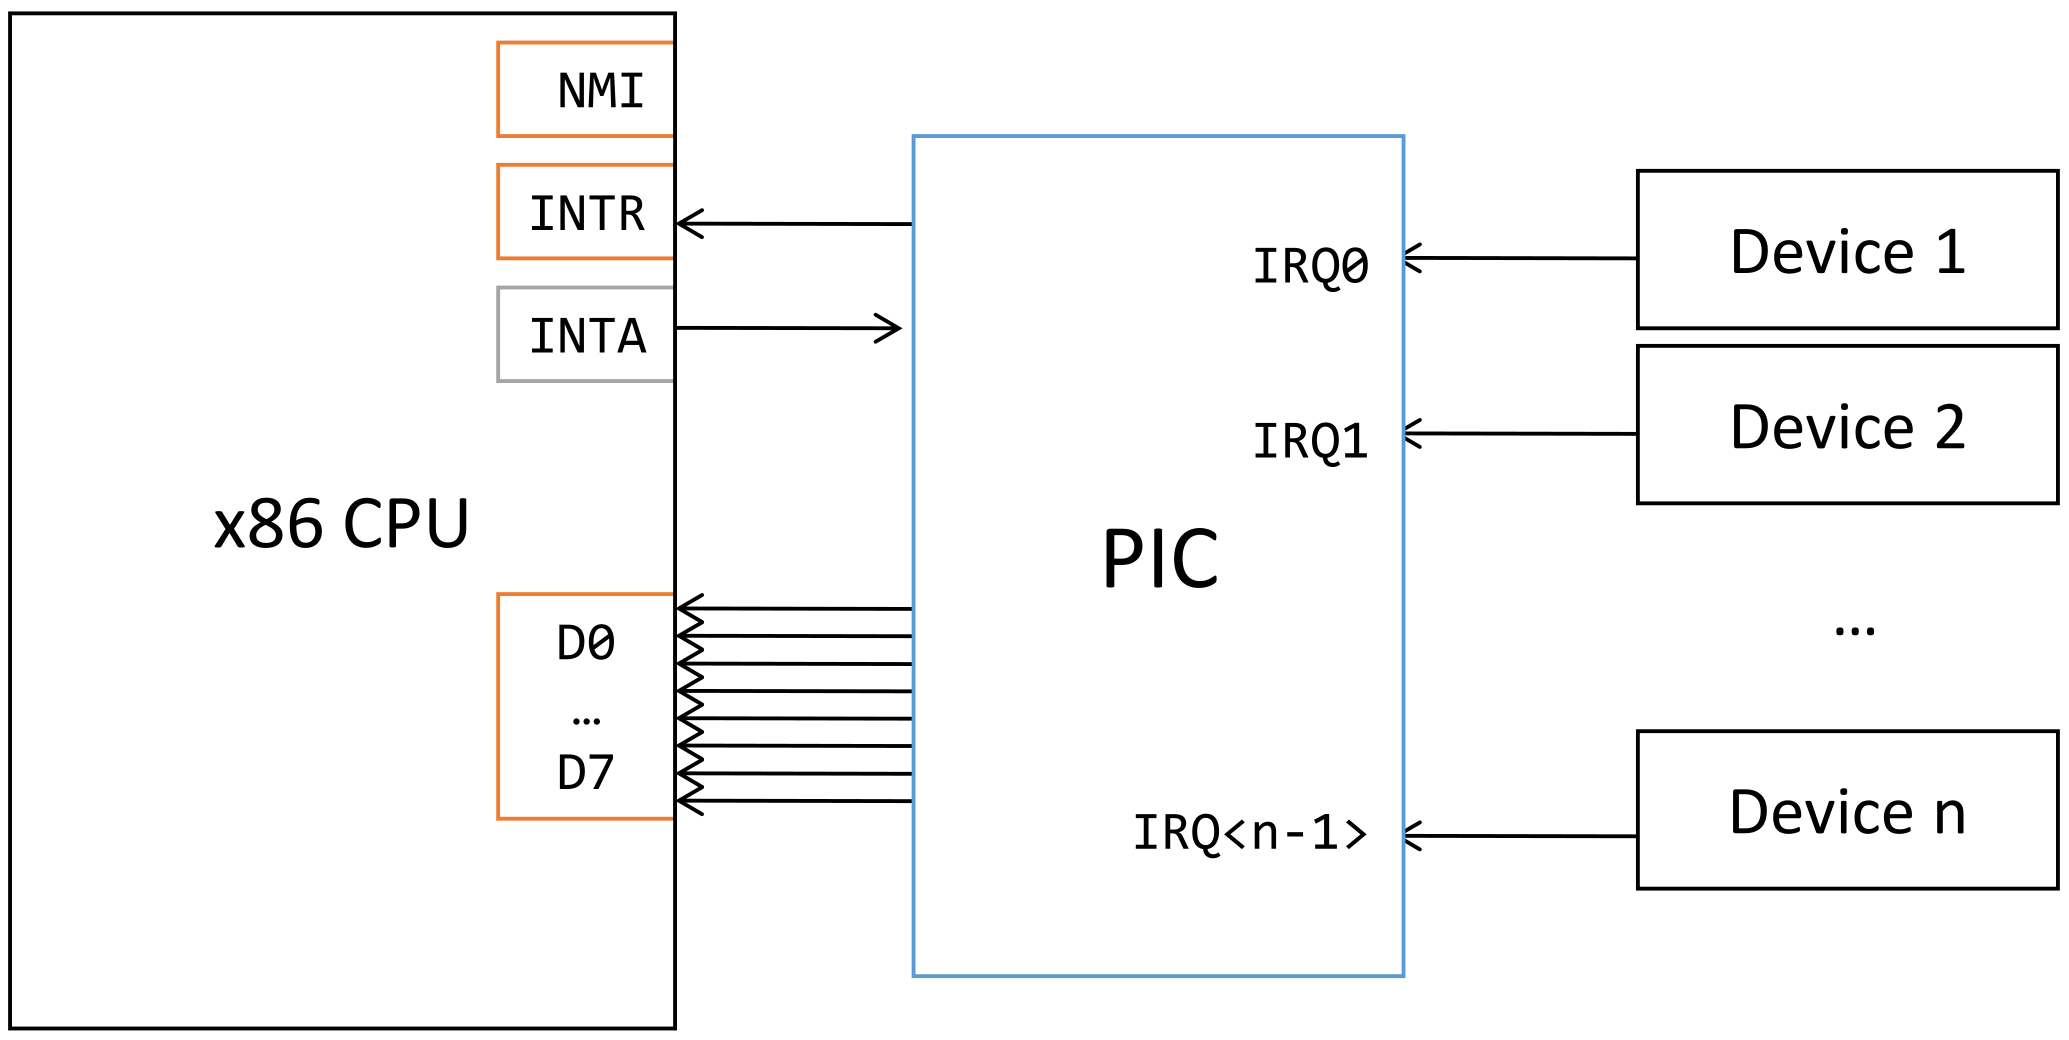
\includegraphics[width=0.8\textwidth]{19_Pic.png}

The PIC can also buffer simultaneous interrupts and deliver each interrupt vector separately. It also allows to prioritize devices over others as well as selectively mask any individual device's interrupts.

Over time the PIC was improved and integrated into the processor itself. Also, they support multiple processors systems as used in datacenters. They also have many more advanced features. 

This gets more complex....

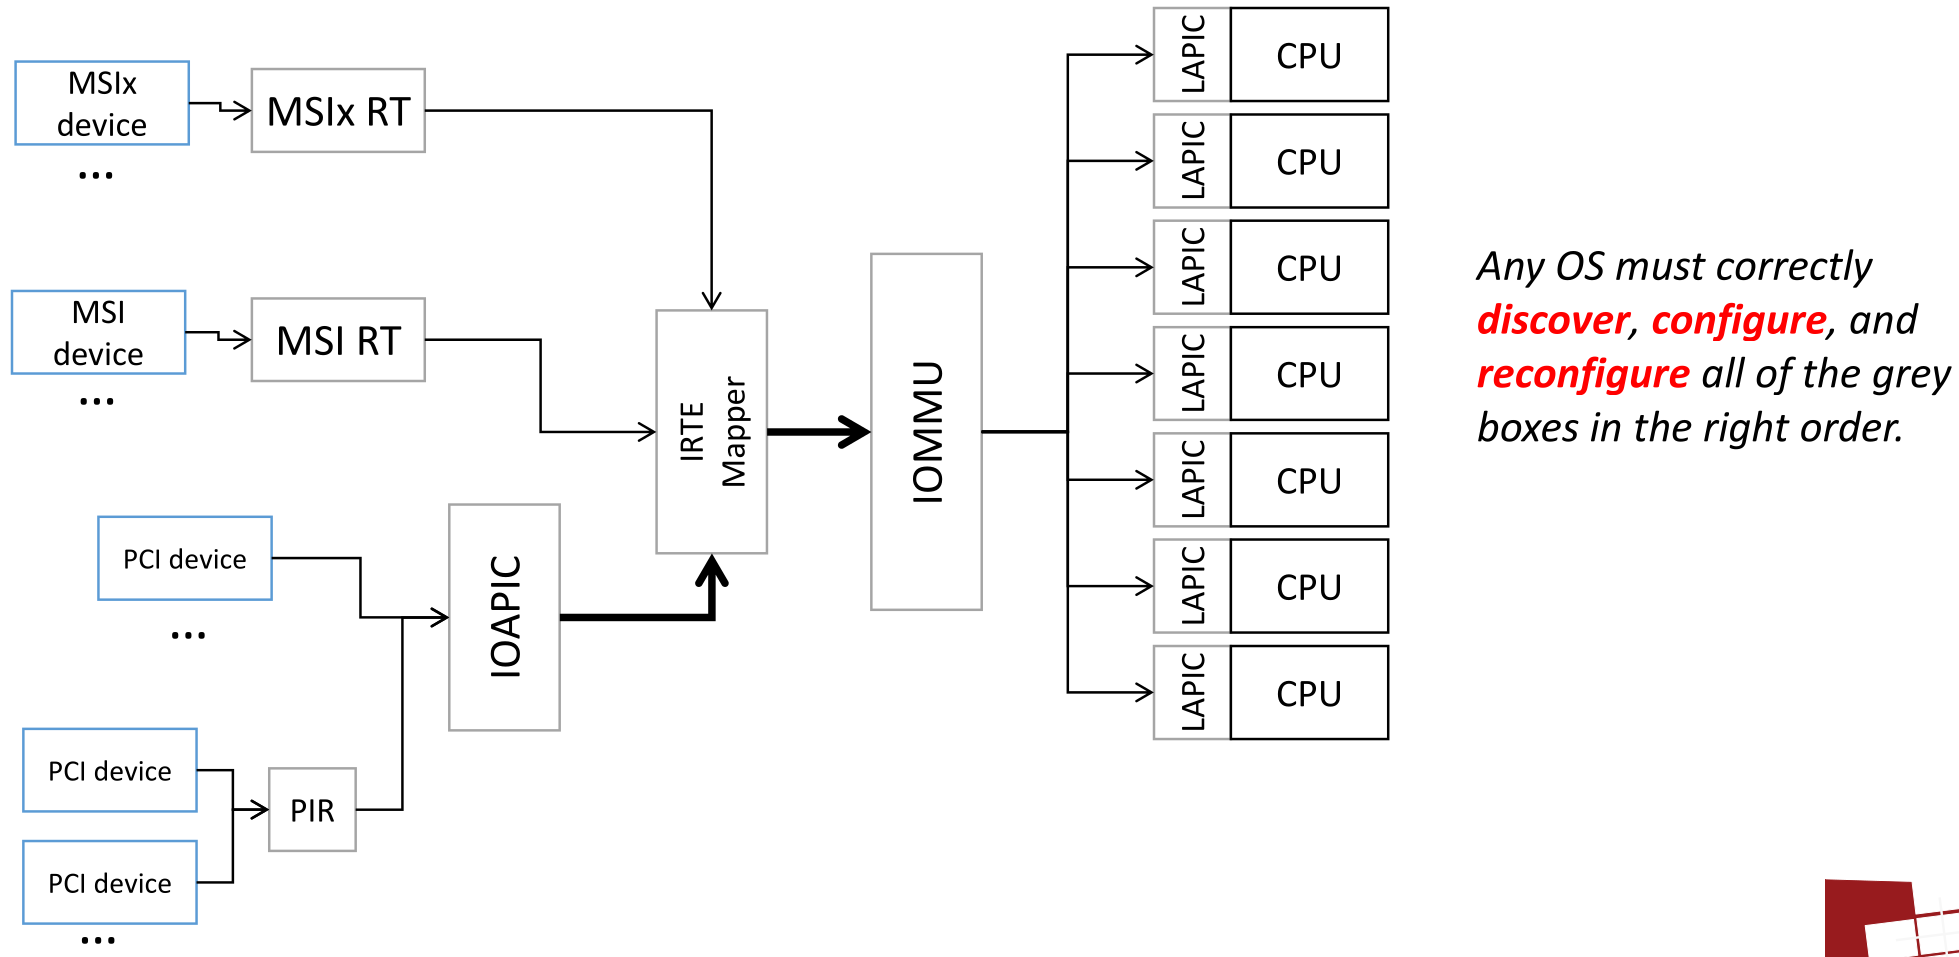
\includegraphics[width=0.8\textwidth]{19_modernPc.png}
